\chapter{Sensitivity of the Model}

A sensitivity analysis considers the extent to which uncertainty in model inputs influences model 
output.  For a sensitivity analysis, this uncertainty includes not only that inherent in the input of 
data for specific scenarios by the model user, but also uncertainty in empirical data or numerical 
parameters in the model such as the time step size used by the model to obtain a solution. 

Among the purposes for conducting a sensitivity analysis are to determine 
\begin{itemize}
\item the important variables in the models, 
\item the computationally valid range of values for each input variable, and 
\item the sensitivity of output variables to variations in input data. 
\end{itemize}

Conducting a sensitivity analysis of a complex model is not a simple task and it will differ 
depending on the application. CFAST typically requires the user to provide numerous input 
parameters that describe the building geometry, compartment connections, construction 
materials, and description of one or more fires. 

Iman and Helton \cite{Iman:1988} studied the sensitivity of complex computer models developed to simulate the risk of severe nuclear accidents which may include fire and other risks. Consistent with the 
work of Iman and Helton \cite{Iman:1988}, ASTM E1355 \cite{ASTM:E1355} provides overall guidance on typical areas of evaluation of the sensitivity of deterministic fire models.  These areas may involve one or more of the following techniques: finite difference or direct analysis methods that provide an explicit solution of the sensitivity equations associated with the governing equations of the model, 
factorial design or Latin hypercube sampling studies that investigate the effect of varying the 
input parameters and consequential interactions between parameters that may be deemed 
important, and global or response surface methods that investigate the overall behavior of model 
outputs for a desired range of inputs. 

This chapter provides a review of the sensitivity studies that have been conducted using CFAST 
with an emphasis on uncertainty in the input. Other sensitivity investigations of CFAST are also 
available \cite{Peacock:1988a, Beard:1992, Notarianni:2000}. 

\section{Factorial Design Studies}

Khoudja [\cite{Khoudja:1988} has studied the sensitivity of an early version of the FAST [2] (predecessor to CFAST) model with a fractional factorial design involving two levels of 16 different input 
parameters. The statistical design, taken from the texts by Box and Hunter \cite{Box:1978}, and Daniel \cite{Daniel:1976} reduced the necessary model runs from more than 65 000 to 256 by studying the interactions of input parameters simultaneously. The choice of values for each input parameter represented a range for each parameter. The analysis of the FAST model showed sensitivity to heat loss to the compartment walls and to the number of compartments in the simulation. Without the inclusion 
of surface thermophysical properties, this model treats surfaces as adiabatic for conductive heat 
transfer. Thus, consistent sensitivity should be expected. Sensitivity to changes in thermal 
properties of the surfaces were not explored. 

Walker \cite{Walker:1997} discussed the uncertainties in components of zone models and showed how 
uncertainty within user-supplied data affects the results of calculations using CFAST as an 
example. The study systematically varied inputs related to the fire (heat release rate, heat of 
combustion, mass loss rate, radiative fraction, and species yields) and compartment geometry 
(vent size and ceiling height) ranging from  $\pm$ 1 \% to $\pm$ 20 \% of base values for a one- 
compartment scenario. Heat release rate and ceiling height are seen to be the dominant input 
variables in the simulations. Upper layer temperature changed $\pm$ 10 \% for a $\pm$ 10 \% change in 
heat release rate. Typical variation of $\pm$ 10 s in time to untenable conditions for a 20 \% variation 
in the inputs was noted for the scenarios studied. 

Peacock et al. \cite{Peacock:1988a} studied the sensitivity of CFAST for a range of input parameters. They used simple factorial designs for model inputs deemed important to investigate local behavior of 
important model outputs along with response surface methods to evaluate overall model 
behavior. Results of the parametric investigations are discussed below and the application of 
response surface methods is summarized in section 5.2. Both are discussed in more detail in 
reference \cite{Peacock:1988a}.

\subsection{Model Inputs and Outputs}

Most studies of modeling related to fire hazard and fire reconstruction present a consistent set of 
variables of interest to the model user \cite{Emmons:1988, Duong:1990, Beard:1992, NRCNUREG1824Overview} : upper and lower gas layer temperatures, gas species concentrations, and layer interface position. Other variables of interest include 

\begin{itemize}
\item mass pyrolysis and heat release rate, 
\item room pressure, and 
\item vent flow. 
\end{itemize}

Although there are certainly other comparisons of interest, these will provide evidence of the 
sensitivity of the model to most model inputs.  Tables 4 and 5 show typical inputs and outputs 
for the CFAST model.

\begin{table}
\begin{center}
\caption{Typical Inputs for a Two-Zone Fire Model}
\label{tab:Two_Zone_Inputs}
\begin{tabular}{| c | c | c | c | c | c | c | c |}
\hline
\multirow{2}{*}{Surface} & $b_1$ & $b_2$ & $b_3$ & $b_4$ & $b_5$ & $b_6$ & $b_7$ \\
 & (m) & (m\superscript{3}/kg) & (s\superscript{-1}) & (J/g mol) & (m\superscript{3}/kg)\superscript{$b_7 - b_6$} & (note a) & (note b) \\ 
 \hline
 Painted Gypsum & 0.0063 & 191.8 & 0.0587 & 7476 & 193 & 1.021 & 0.431 \\ \hline
 PMMA & $9.6 x 10^{-5}$ & 0.0137 & 0.0205 & 7476 & 29 & 1.0 & 0.431 \\ \hline
 Ceiling Tile & $4.0 x 10^{-3}$ & 0.0548 & 0.123 & 7476 & 30\superscript{a} & 1.0 & 0.431 \\ \hline
 Cement Block & $1.8 x 10^{-2}$ & 5.48 & 0.497 & 7476 & 30\superscript{a} & 1.0 & 0.431 \\  \hline
 Calcium Silicate Board & $1.9 x 10^{-2}$ & 0.137 & 0.030 & 7476 & 30\superscript{a} & 1.0 & 0.431 \\  \hline
\end{tabular}
\end{center}
a - very approximate value, insufficient data for high confidence value

b - non-dimensional
\end{table}

\begin{table}
\begin{center}
\caption{Typical Outputs for a Two-Zone Fire Model}
\label{tab:Two_Zone_Outputs}
\begin{tabular}{| c | c | c | c | c | c | c | c |}
\hline
\multirow{2}{*}{Surface} & $b_1$ & $b_2$ & $b_3$ & $b_4$ & $b_5$ & $b_6$ & $b_7$ \\
 & (m) & (m\superscript{3}/kg) & (s\superscript{-1}) & (J/g mol) & (m\superscript{3}/kg)\superscript{$b_7 - b_6$} & (note a) & (note b) \\ 
 \hline
 Painted Gypsum & 0.0063 & 191.8 & 0.0587 & 7476 & 193 & 1.021 & 0.431 \\ \hline
 PMMA & $9.6 x 10^{-5}$ & 0.0137 & 0.0205 & 7476 & 29 & 1.0 & 0.431 \\ \hline
 Ceiling Tile & $4.0 x 10^{-3}$ & 0.0548 & 0.123 & 7476 & 30\superscript{a} & 1.0 & 0.431 \\ \hline
 Cement Block & $1.8 x 10^{-2}$ & 5.48 & 0.497 & 7476 & 30\superscript{a} & 1.0 & 0.431 \\  \hline
 Calcium Silicate Board & $1.9 x 10^{-2}$ & 0.137 & 0.030 & 7476 & 30\superscript{a} & 1.0 & 0.431 \\  \hline
\end{tabular}
\end{center}
a - very approximate value, insufficient data for high confidence value

b - non-dimensional
\end{table}

Consider the following fire scenario: The building geometry (figure \ref{fig:Sensitivity_BaseCase}) includes four rooms on two floors with horizontal, vertical, and mechanical vents connecting the rooms and venting to the outdoors. The fire source in one of the rooms on the lower floor is a medium growth rate t-squared fire \cite{NFPA72:2003} chosen to simulate a mattress fire \cite{Babrauskas:1985}.

\begin{figure}[t]
\begin{center}
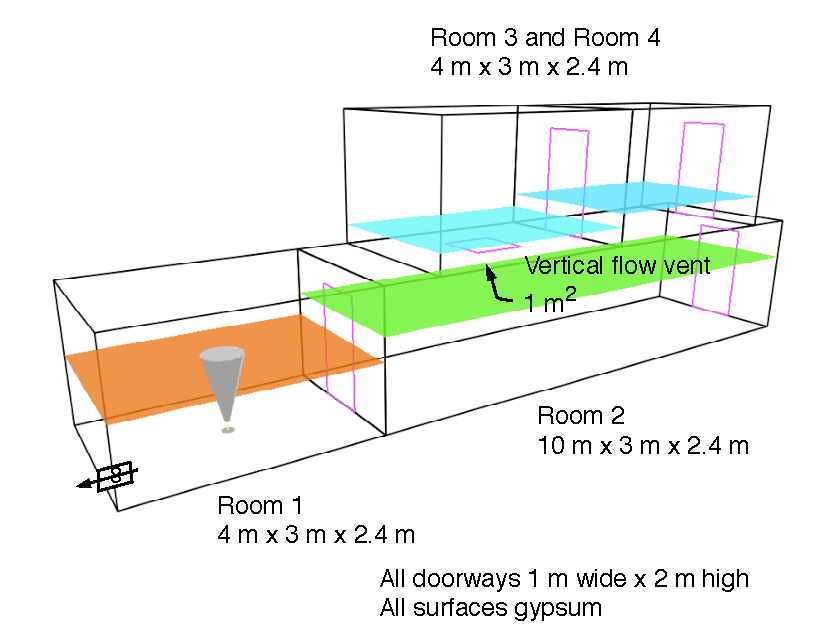
\includegraphics[width=4.5in]{FIGURES/Sensitivity/SensitivitySample}\\
\end{center}
\caption{Building Geometry for base case scenario.}
 \label{fig:Sensitivity_BaseCase}
\end{figure}
